\documentclass[12pt,letterpaper]{article}
\usepackage{fullpage}
\usepackage[top=2cm, bottom=4.5cm, left=2.5cm, right=2.5cm]{geometry}
\usepackage{amsmath,amsthm,amsfonts,amssymb,amscd}
\usepackage{lastpage}
\usepackage{enumerate}
\usepackage{fancyhdr}
\usepackage{mathrsfs}
\usepackage{xcolor}
\usepackage{graphicx}
\usepackage{listings}
\usepackage{hyperref}
\usepackage{amsmath}
\usepackage{mathtools}
\usepackage{tikz}
\usepackage{array}
\usetikzlibrary{matrix}

\hypersetup{%
  colorlinks=true,
  linkcolor=blue,
  linkbordercolor={0 0 1}
}
 
\renewcommand\lstlistingname{Section}
\renewcommand\lstlistlistingname{Algorithms}
\def\lstlistingautorefname{Alg.}

\lstdefinestyle{Python}{
    language        = Python,
    frame           = lines, 
    basicstyle      = \footnotesize,
    keywordstyle    = \color{blue},
    stringstyle     = \color{green},
    commentstyle    = \color{red}\ttfamily
}

\setlength{\parindent}{0.0in}
\setlength{\parskip}{0.05in}

% Edit these as appropriate
\newcommand\course{CSE 3500}
\newcommand\hwnumber{3}                  % <-- homework number
\newcommand\NetIDa{rjf23002}           % <-- NetID of person #1
\newcommand\NetIDb{}           % <-- NetID of person #2 (Comment this line out for problem sets)

\pagestyle{fancyplain}
\headheight 35pt
\lhead{\NetIDa}
\lhead{\NetIDa\\\NetIDb}                 % <-- Comment this line out for problem sets (make sure you are person #1)
\chead{\textbf{\Large Homework \hwnumber}}
\rhead{\course \\ \today}
\lfoot{}
\cfoot{}
\rfoot{\small\thepage}
\headsep 1.5em

\begin{document}

\section*{Problem 0}

\item

\lstset{caption={Maximum Cost Path}}
    \lstset{label={lst:alg1}, numbers=left}
    \begin{lstlisting}[style = Python]
        def max_cost_path(grid: list[list]) -> int:
            N = len(grid)
            # prev row's dp values
            dp = [0] * N
            
            for r in range(N):
                # curr row's dp values
                temp = [0] * N
                prev_left = 0
                for c in range(N):
                    # normal path dp, go two directions (down, right)
                    # either curr val, or top, or left
                    temp[c] = max(dp[c], prev_left) + grid[r][c]
                    prev_left = temp[c]
                
                # prefix sum, traverse backwards (left)
                if r > 0:
                    prefix_sum = 0
                    for c in range(N - 2, -1, -1):
                        if r > 0:
                            prefix_sum += grid[r - 1][c + 1]
                        prefix_sum += grid[r][c + 1]
                        temp[c] = max(temp[c], temp[c] + prefix_sum)
                
                dp = temp
        
            return dp[-1]
\end{lstlisting}

Since there are negative edges, we cannot use Dijkstra's algo.
We also can't use BFS as it will only find us the minimum length path, 
and not the max cost path.
To solve the max cost path, we can go in two directions first. (One vertical and one horizontal).
Here, we choose to go downwards and rightwards first.
Hence, at an arbitrary cell, 
the maximum cost is either the max from the top (dp[c]) or the value from the left (prev left) + the grid cost.
If we iterate in this way, we will find the maximum cost path
just by going downwards and rightwards at the end of the last iteration. \\

However, in this question, we need to consider left paths as well.
We can do so at every step using a prefix sum.
This lets us consider the diagonal right and rightside values.
We cache this value and can reuse it for future subproblems.

\newpage

\section*{Problem 1}

We can use divide and conquer to solve this problem, applying a similar technique to merge sort.
Instead of dealing with n crows, we can instead break it up into two halves of similar length n/2 crows. 
We keep breaking it up until we have small chunks of size 1 or no birds, which is our base case.
Once we have obtained our base cases, we can then do the rebuilding/ combining step, similar to merge sort. \\

In the combining step, we can categorize our crows and find the identical crows at the same time.
For example, given just two crows from the base case, we can call the operation (let's call it OP) to find out if they are similar.
Let us first form two categories: Identical and non identical.
We can then maintain two lists of crows, one for each category.
After performing OP on the two crows, 
we can append them to their respective lists, and continue combining with larger cases. 
At larger cases, we perform the same action. 
Assume we have identical (i1, i2) and non-identical lists (j1, j2).
We can simply append the new identical to be i1 + j1 since there aren't multiple sets of identical birds.
We can do the same for the non-identical birds i2 + j2.
As there aren't multiple sets of identical birds, we can avoid performing OP.
\\

Hence, at the end of the algorithm, we can then check our two lists.
We are able to check our list of identical crows to see if it
contains more than n/2 crows to solve the problem. \\

Runtime: 
For a problem size of n, we split it into 2 subproblems of size n/2 recursively. 
This gives the relationship of subproblems to be T(n) = 2T(n/2).
For the merging step, we iteratively go through the subarrays of combined sizes n, n/2, n/4, ..., n/k such that n/k = 1.
Hence, at each an arbitrary level k, we do O(n/k) amount of work for the merge. 
Thus, the final recurrence can be given by T(n) = 2T(n/2) + O(n). 
Therefore, at each level, we do O(n) amount of work.
Given that there are $log_2 n$ levels, the time complexity is hence bounded by O(nlogn).

\newpage

\section*{Problem 2}
The algorithm in hand can be compared to bubble sort as swapping occurs between neighbours.
The only difference would be that choosing which element to swap is done arbitrarily and not in order.
For our algorithm, we can say that a single swap operation resolves one sorted pair of elements,
simply because it swaps them to the right order.
Thus, we can say that it eliminates one swap operation from the whole sorting sequence.
That is, we won't ever need to swap these two again and they can be marked as resolved.
As an array has a finite number of steps to be sorted, by repeatedly running our swap function, 
we won't run into a pair we have encountered before.
Thus, the number of unresolved pairs will keep decreasing by one, until eventually hit 0 unresolved pairs.
At this stage, the array is sorted. \\

Invariants: Every swap operations causes the total number of unsorted pairs to decrease by one.

\newpage

\section*{Problem 3}

\begin{enumerate}
    \item 
    An example array would be [1, 2, 3, 4, 5, 6, 7]. \\
    
    Build max heap originally starts off with the heap:
    \begin{figure}[!h]
      \centering
      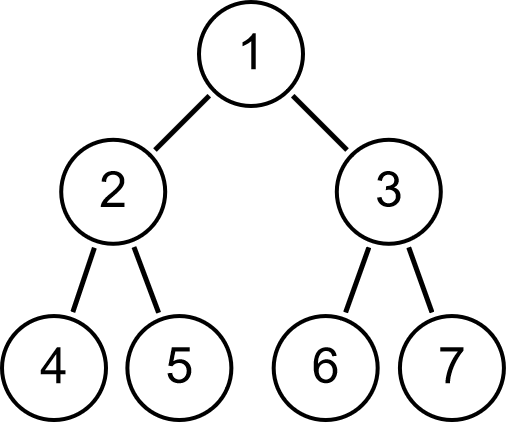
\includegraphics[width=0.2\linewidth]{mh1_before.png}
      \end{figure}
      
    And ends up as this:
    \begin{figure}[!h]
      \centering
      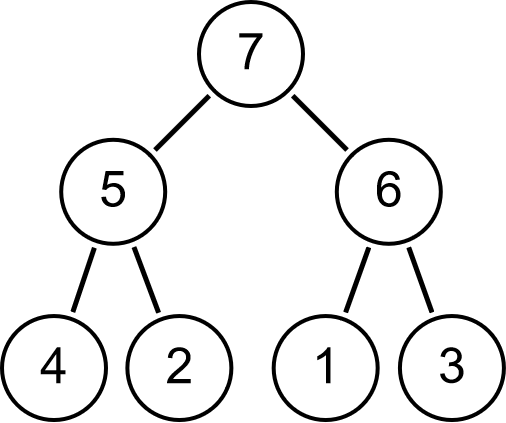
\includegraphics[width=0.2\linewidth]{mh1_after.png}
      \end{figure}
      
    Build max heap 2 gets us this heap:
    \begin{figure}[!h]
      \centering
      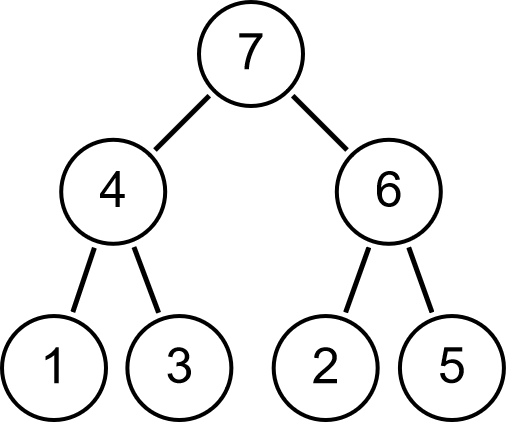
\includegraphics[width=0.2\linewidth]{mh2_after.png}
      \end{figure}
      
    \item 
    O(nlogn). 
    The maxheapinsert operation just inserts a single element into the heap. 
    If the element is not in the right position, we just perform a swap.
    Performing a swap is just a simple operation of changing the pointers.
    Hence, it is O(1). We potentially have to go down log(n) levels, 
    hence the cost of it is log(n) just for a single operation.
    As we perform it n times, it is O(nlogn).

\end{enumerate}

\end{document}
